\documentclass[11pt]{article}

\usepackage{fancyhdr}
\usepackage{graphicx}
\usepackage{geometry}
\usepackage{lastpage}
\usepackage{titling}
\usepackage{sectsty}
\usepackage{setspace}
\usepackage{changepage}
\usepackage[shortlabels]{enumitem}
\usepackage{subcaption}
\usepackage{helvet}

\usepackage{siunitx}
\usepackage{nicefrac}
\usepackage{amsmath}
\usepackage{gensymb}
\usepackage{amssymb}
\usepackage{float}

\usepackage{listings}
\usepackage{color}
\definecolor{dkgreen}{rgb}{0,0.6,0}
\definecolor{gray}{rgb}{0.5,0.5,0.5}
\definecolor{mauve}{rgb}{0.58,0,0.82}

\lstset
{
  frame=tb,
  language=MATLAB,
  aboveskip=3mm,
  belowskip=3mm,
  showstringspaces=false,
  columns=flexible,
  basicstyle={\small\ttfamily},
  numbers=none,
  numberstyle=\tiny\color{gray},
  keywordstyle=\color{blue},
  commentstyle=\color{dkgreen},
  stringstyle=\color{mauve},
  breaklines=true,
  breakatwhitespace=true,
  tabsize=3
}

\geometry
{
  letterpaper, 
  total={175.9mm,229.4mm}, 
  top=25mm, 
  left=20mm, 
  headheight=15pt,
  voffset=12pt,
  footskip=15pt
}
\author{Daniel Sturdivant}
\title{Homework 1}
\date{January 2023}
\graphicspath{ {./media/} }

\pagestyle{fancy}
\fancyhead[R]{January 30, 2023}
\fancyhead[L]{Sturdivant, Daniel}
\fancyhead[C]{MECH 7710 Optimal}
\fancyfoot[C]{Page \thepage\ of \pageref{LastPage}}

\makeatletter
\def\@maketitle
{
  \null
  \begin{center}
    {\huge \@title \\}
  \end{center}
  \vskip 5mm
}
\makeatother

\sectionfont{\fontsize{16}{16}}
\subsectionfont{\fontsize{13}{13}\normalfont}
\renewcommand{\thesubsection}{\arabic{section}-\arabic{subsection}}
\renewcommand{\familydefault}{\sfdefault}
\newcommand{\solution}{\textbf{Solution: \\}}


%% ====================================================================== %%
\begin{document}

\maketitle
\thispagestyle{fancy}
\setstretch{1.25}
% \setlength{\parskip}{0em}
% \setlength{\abovedisplayskip}{-8pt}
% \setlength{\belowdisplayskip}{12pt}
\setlength{\parindent}{0pt}

\begin{enumerate}[label=\textbf{\arabic*.}]
  \itemsep 12pt
  % problem 1
  \item A control law for a simple rotation table is to be designed. The table 
  has a rotational moment of inertia ($J$) of 10 kg-m2 and rotational damping 
  ($b$) of 1 N-m-s/rad. Torque is commanded to the motor and the table’s position 
  is measured using a rotary encoder.
  \begin{enumerate}[(a)]
    \itemsep -6pt
    \item Derive the simple differential equation for the system.
    \item Convert the system into a state-space format.
    \item What are the eigenvalues of the system.
  \end{enumerate}
  \solution
  \begin{figure}[H]
    \centering
    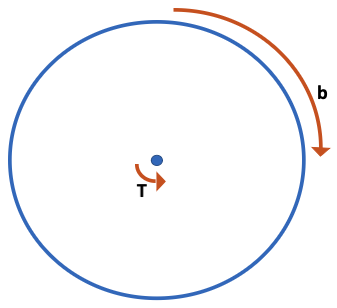
\includegraphics[width=0.3\textwidth]{p1.png}
    \caption{System Diagram.}
  \end{figure}

  Summing the moments on the table.
  \begin{equation}
    \begin{split}
      \sum M &= J \ddot{\theta} = T - b \dot{\theta} \\
      &= 10 \ddot{\theta} = T - 1 \dot{\theta} \\
      T &= 10 \ddot{\theta} + \dot{\theta}
    \end{split}
  \end{equation}

  Linearizing the system and putting it in matrix form.
  \begin{equation}
    \begin{split}
      \begin{bmatrix} 
        x_1 \\ x_2 
      \end{bmatrix}
      &= 
      \begin{bmatrix}
        \theta \\ \dot{\theta}
      \end{bmatrix}
      \\
      \begin{bmatrix} 
        \dot{x_1} \\ \dot{x_2} 
      \end{bmatrix}
      &= 
      \begin{bmatrix}
        \dot{\theta} \\ \ddot{\theta}
      \end{bmatrix}
      =
      \begin{bmatrix}
        x_2 \\ 0.1(u - x_2)
      \end{bmatrix}
      =
      \begin{bmatrix}
        \dot{\theta} \\ 0.1(T - \dot{\theta})
      \end{bmatrix}
      \\
      y &= \theta
    \end{split}
  \end{equation}

  Formulating the state space equations.
  \begin{equation}
    \begin{split}
      \dot{x} &= Ax + Bu \\
      \begin{bmatrix}
        \dot{\theta} \\ \ddot{\theta}
      \end{bmatrix}
      &= 
      \begin{bmatrix}
        0 & 1 \\ 0 & -0.1
      \end{bmatrix}
      \begin{bmatrix}
        \theta \\ \dot{\theta}
      \end{bmatrix}
      +
      \begin{bmatrix}
        0 \\ 0.1
      \end{bmatrix}
      T
    \end{split}
  \end{equation}

  \begin{equation}
    \begin{split}
      y &= Cx \\
      \begin{bmatrix}
        y
      \end{bmatrix}
      &=
      \begin{bmatrix}
        1 & 0
      \end{bmatrix}
      \begin{bmatrix}
        \theta \\ \dot{\theta}
      \end{bmatrix}
    \end{split}
  \end{equation}

  Solving for the eigenvalues of the open-loop system.
  \begin{equation}
    \begin{split}
      0 &= det(sI - A) \\
      0 &= det
      \begin{bmatrix}
        s & -1 \\ 0 & s+0.1
      \end{bmatrix} \\
      0 &= s(s+0.1) \\
      s &= 0, -0.1
    \end{split}
  \end{equation}

  % problem 2
  \vspace{24pt}
  \item Design an observer for the above system.
  \begin{enumerate}[(a)]
    \itemsep -6pt
    \item Show that the system is observable.
    \item Design $L$ such that the error dynamics have $f_n=50$ Hz and $\zeta=0.7$.
    \item Provide a plot of the step response of the estimator.
  \end{enumerate}
  \solution

  To determine the observability of the system, the rank of the observability 
  matrix is checked. For this system this must equal 2 (the dimension of A).
  \begin{equation}
    \begin{split}
      \mathcal{O} &= 
      \begin{bmatrix}
        C \\ CA
      \end{bmatrix}
      = 
      \begin{bmatrix}
        1 & 0 \\ 0 & 1
      \end{bmatrix}
    \end{split}
  \end{equation}

  \begin{equation}
    rank(\mathcal{O}) = 2
  \end{equation}

  The system is observable and the poles of the observer can be placed using the 
  dynamics defined.
  \begin{equation}
    \begin{split}
      0 &= s^2 + 2 \omega_n \zeta s + \omega_n^2 \\
      0 &= s^2 + 2 (2 \pi f_n) \zeta s + (2 \pi f_n)^2 \\
      0 &= s^2 + 2 (100 \pi) 0.7 s + (100 \pi)^2 \\
      s &= -219.91 \pm 224.35i = s_{obsv}
    \end{split}
  \end{equation}

  \begin{equation}
    L = place(A', C', s_{obsv})' =
    \begin{bmatrix}
      439.72 \\ 98652.08
    \end{bmatrix}
  \end{equation}

  The new closed-loop A matrix.
  \begin{equation}
    A_{obsv} = A-LC =
    \begin{bmatrix}
      -439.72 & 1 \\ -98652.08 & -0.1
    \end{bmatrix}
  \end{equation}

  \begin{figure}[H]
    \centering
    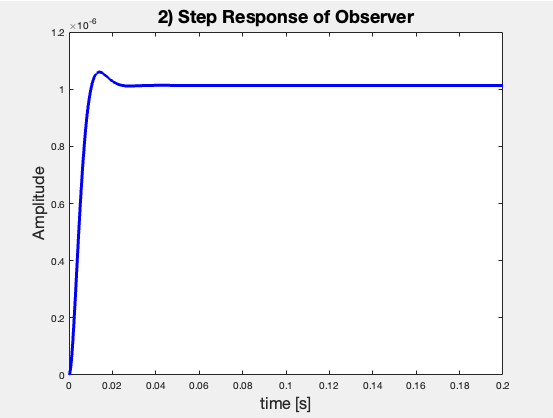
\includegraphics[width=0.6\textwidth]{p2.png}
    \caption{Observer Step Response.}
  \end{figure}

  % problem 3
  \vspace{24pt}
  \item Design a state-feedback controller for the table.
  \begin{enumerate}[(a)]
    \itemsep -6pt
    \item Show that the system is controllable.
    \item Design $K$ such that $f_n=10$ Hz and $\zeta=0.7$.
    \item Provide a plot of the step response of the combined estimator and controller.
  \end{enumerate}
  \solution

  To determine the controllability of the system, the rank of the controllability 
  matrix is checked. For this system this must equal 2 (the dimension of A).
  \begin{equation}
    \mathcal{C} = 
    \begin{bmatrix}
      B & AB
    \end{bmatrix}
    =
    \begin{bmatrix}
      0 & 0.1 \\ 0.1 & -0.01
    \end{bmatrix}
  \end{equation}

  \begin{equation}
    rank(\mathcal{C}) = 2
  \end{equation}

  The system is controllable and the poles of the controller can be placed using the 
  dynamics defined.
  \begin{equation}
    \begin{split}
      0 &= s^2 + 2 \omega_n \zeta s + \omega_n^2 \\
      0 &= s^2 + 2 (2 \pi f_n) \zeta s + (2 \pi f_n)^2 \\
      0 &= s^2 + 2 (20 \pi) 0.7 s + (20 \pi)^2 \\
      s &= -43.98 \pm 44.87i = s_{cont}
    \end{split}
  \end{equation}

  \begin{equation}
    K = place(A, B, s_{cont}) =
    \begin{bmatrix}
      39478.40 & 878.65
    \end{bmatrix}
  \end{equation}

  The new combined closed-loop system.
  \begin{equation}
    \begin{split}
      A &= 
      \begin{bmatrix}
        A-BK & BK \\ 0 & A-LC
      \end{bmatrix}
      =
      \begin{bmatrix}
        0 & 1 & 0 & 0 \\
        -3947.84 & -87.96 & 3947.84 & 87.86 \\
        0 & 0 & -439.72 & 1 \\
        0 & 0 & -98652.07 & -0.1
      \end{bmatrix} \\
      B &=
      \begin{bmatrix}
        B \\ 0
      \end{bmatrix}
      =
      \begin{bmatrix}
        0 \\ 0.1 \\ 0 \\ 0
      \end{bmatrix} \\
      C &=
      \begin{bmatrix}
        C & 0
      \end{bmatrix}
      =
      \begin{bmatrix}
        1 & 0 & 0 & 0
      \end{bmatrix} \\
      D &= 0
    \end{split}
  \end{equation}
  \begin{figure}[H]
    \centering
    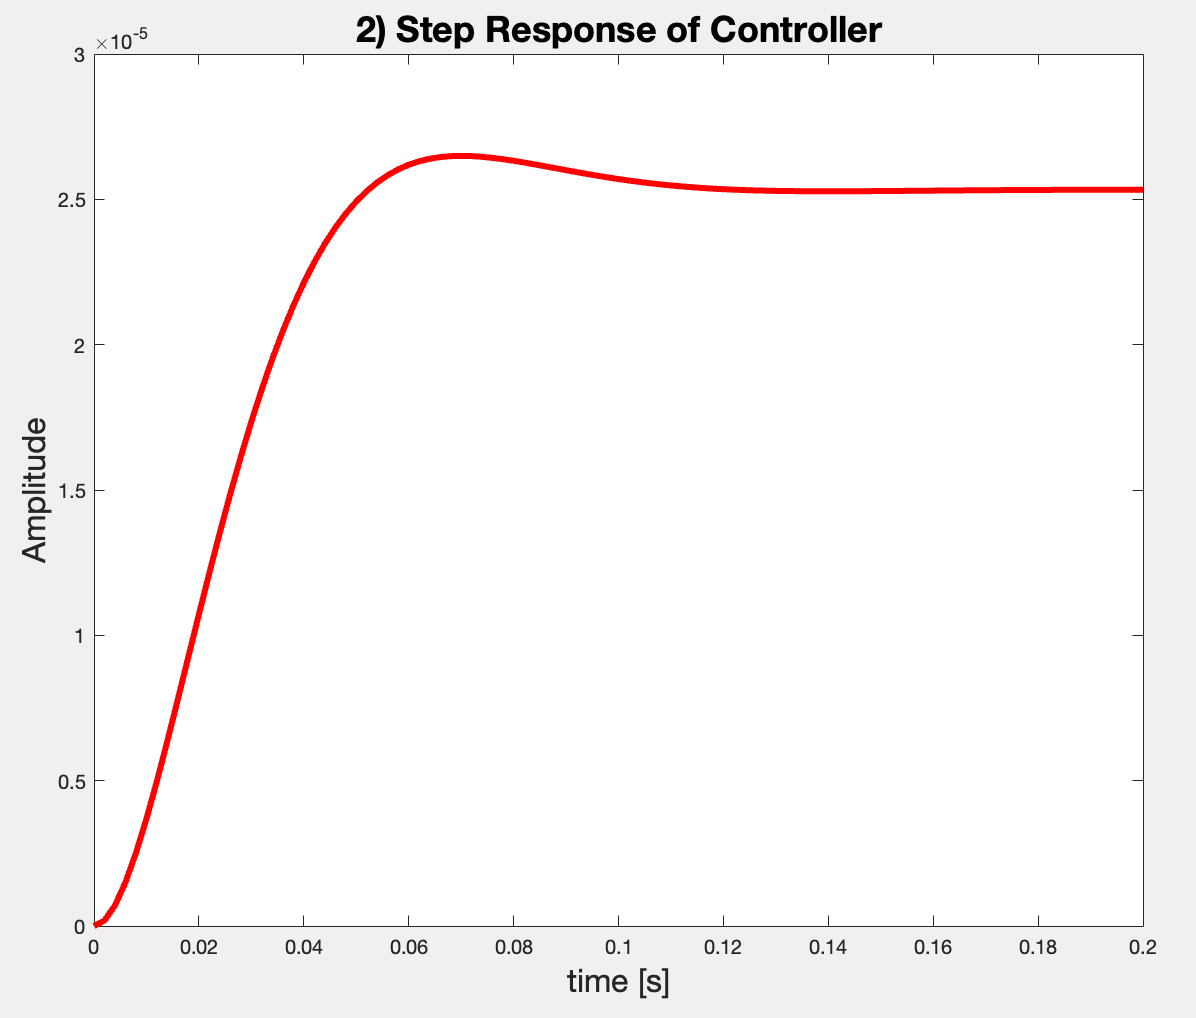
\includegraphics[width=0.6\textwidth]{p3.png}
    \caption{Combined Controller and Observer Step Response.}
  \end{figure}

  % problem 4
  \vspace{24pt}
  \item Solve for the equivalent compensator for the system.
  \begin{enumerate}[(a)]
    \itemsep -6pt
    \item What kind of classical compensator does it resemble?
    \item Calculate the closed loop transfer function.
    \item Plot the Bode Plot of the closed-loop system.
    \item Find the gain and phase margin.
  \end{enumerate}
  \solution

  Transforming the controller and observer defined above into an equivalent 
  compensator results in the following system.
  \begin{equation}
    \begin{split}
      A_{comp} &= A - BK - LC =
      \begin{bmatrix}
        -439.72 & 1 \\ -102599.92 & -87.96
      \end{bmatrix} \\
      B_{comp} &= L =
      \begin{bmatrix}
        439.72 \\ 98652.08
      \end{bmatrix} \\
      C_{comp} &= K =
      \begin{bmatrix}
        39478.40 & 878.65
      \end{bmatrix}
    \end{split}
  \end{equation}

  With an equivalent transfer function of:
  \begin{equation}
    \begin{split}
      \dfrac{U(s)}{Y(s)} & = C_{comp}(sI-A_{comp})^{-1}B_{comp} 
      = -K(sI - A + BK + LC)^{-1}L \\
      &= \dfrac{-1.04(10^8)s - 3.896(10^9)}{s^2 + 527.7s + 1.413(10^5)}
    \end{split}
  \end{equation}

  This resembles a "lead-lag" compensator because of the extra pole in the 
  denominator (first order numerator, second order denominator). The new system 
  looks like the following when $r=0$ which in turn makes $e=-y$ and 
  $\dfrac{U(s)}{E(s)} = -\dfrac{U(s)}{Y(s)}$.

  \begin{figure}[H]
    \centering
    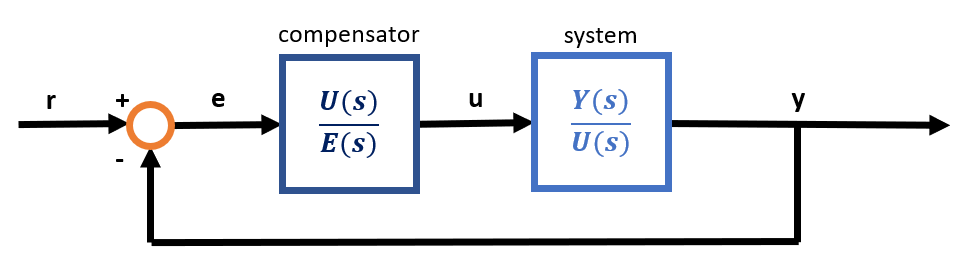
\includegraphics[width=0.5\textwidth]{p4-1.png}
    \caption{System diagram with Compensator.}
  \end{figure}

  To close the loop between the compensator and the plant the following state 
  space system is applied.
  \begin{equation}
    \begin{split}
      A_{cl} =
      \begin{bmatrix}
        A & BC_{comp} \\ -B_{comp}C & A_{comp}
      \end{bmatrix} 
      &=
      \begin{bmatrix}
        0 & 1 & 0 & 0 \\ 
        0 & -0.1 & 3947.84 & 87.86 \\ 
        -439.72 & 0 & -439.72 & 1 \\
        -98652.08 & 0 & 102599.92 & -87.96
      \end{bmatrix} \\
      B_{cl} &= 
      \begin{bmatrix}
        0 \\ B_{comp}
      \end{bmatrix} 
      =
      \begin{bmatrix}
        0 \\ 0 \\ 439.72 \\ 98652.08
      \end{bmatrix} \\
      C_{cl} &=
      \begin{bmatrix}
        C & 0
      \end{bmatrix}
      =
      \begin{bmatrix}
        1 & 0 & 0 & 0
      \end{bmatrix} \\
      D_{cl} &= 0
    \end{split}
  \end{equation}

  Plotting the Bode Plot for the closed-loop system.
  \begin{figure}[H]
    \centering
    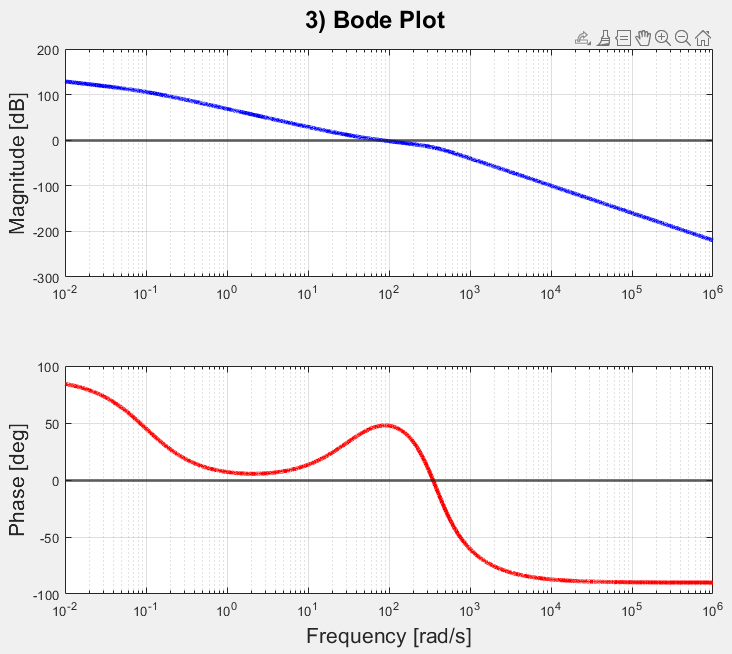
\includegraphics[width=0.6\textwidth]{p4.png}
    \caption{Closed-Loop Compensator Bode Plot.}
  \end{figure}

  Using the MATLAB function $margin$, the gain and phase margin are easily 
  calculated and can be confirmed by analyzing the Bode Plot above.
  \begin{equation}
    \begin{split}
      G_m &= 14.26 \:\si{dB} \\
      \phi_m &= 94.69 \:\si{\degree}
    \end{split}
  \end{equation}

  % problem 5
  \vspace{24pt}
  \item Design the controller in the discrete domain assuming a 1 KHz sample rate.
  \begin{enumerate}[(a)]
    \itemsep -6pt
    \item Discretize the state space model. Where are the eigenvalues?
    \item Design L to provide the same response as problem 2.
    \item Design K to provide the same response as problem 3.
    \item Where are the closed-loop estimator and controller poles located?
    \item Solve for the equivalent compensator transfer function.
  \end{enumerate}
  \solution

  To discretize the continuous model, the MATLAB function $c2d$ was used in 
  combination with $ss$ to transform the continuous model into state-space.
  \begin{equation}
    \begin{split}
      sys &= c2d(ss(A,B,C,D), 1/1000) \\
      A_z &= 
      \begin{bmatrix}
        1 & 0.001 \\ 0 & 0.999
      \end{bmatrix} \\
      B_z &= 
      \begin{bmatrix}
        5(10^-8) \\ 1(10^-4)
      \end{bmatrix} \\
      C_z &=
      \begin{bmatrix}
        1 & 0
      \end{bmatrix} \\
      D_z &= 0
    \end{split}
  \end{equation}

  To find the discrete poles, $s_{obsv}$ and $s_{cont}$ must be converted to 
  discrete poles.
  \begin{equation}
    \begin{split}
      z &= e^{sT} \\ 
      z_{obsv} &= e^{s_{obsv}*T} = e^{(-219.91 \pm 224.35i)*1/1000}
      = 0.7825 \pm 0.1786i \\
      z_{cont} &= e^{s_{cont}*T} = e^{(-43.98 \pm 44.87i)*1/1000}
      = 0.9560 \pm 0.0429i \\
    \end{split}
  \end{equation}
  \begin{figure}[H]
    \centering
    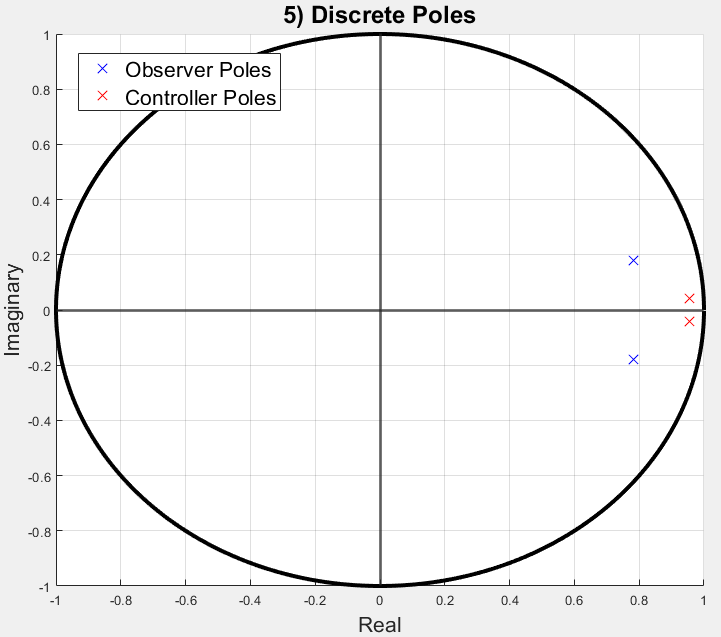
\includegraphics[width=0.5\textwidth]{p5.png}
    \caption{Discrete Pole Placement.}
  \end{figure}

  These new poles can then be used in the MATLAB $place$ function to create the 
  discrete observer and controller.
  \vspace{24pt}
  \begin{equation}
    \begin{split}
      L &= place(A_z', C_z', z_{obsv})' = 
      \begin{bmatrix}
        0.4349 \\ 79.1604
      \end{bmatrix} \\
      K &= place(A_z, B_z, z_{cont}) =
      \begin{bmatrix}
        37781.3243 & 859.9995
      \end{bmatrix}
    \end{split}
  \end{equation}

  Using the same method of finding the compensator transfer function from above:
  \begin{equation}
    \begin{split}
      \dfrac{Y(z)}{U(z)} &= -K_z(zI - A_z + B_zK + L_zC_z)^{-1}L_z \\
      &= \dfrac{-8.451(10^4)z + 8.152(10^4)}{z^2 - 1.477z + 0.594}
    \end{split}
  \end{equation}

  % problem 6
  \vspace{24pt}
  \item Compare the continuous and discrete response using simulation and using 
  equivalent compensator. Plot the simulated and equivalent compensator responses. 
  Compare the expected and actual response. \\ \\ 
  \solution
  Closing the loop for the discrete compensator using $c2d$ on the continuous 
  compensator system.
  \begin{equation}
    sys_{comp_z} = c2d(sys_{comp}, 1/1000)
  \end{equation}

  \begin{figure}[H]
    \centering
    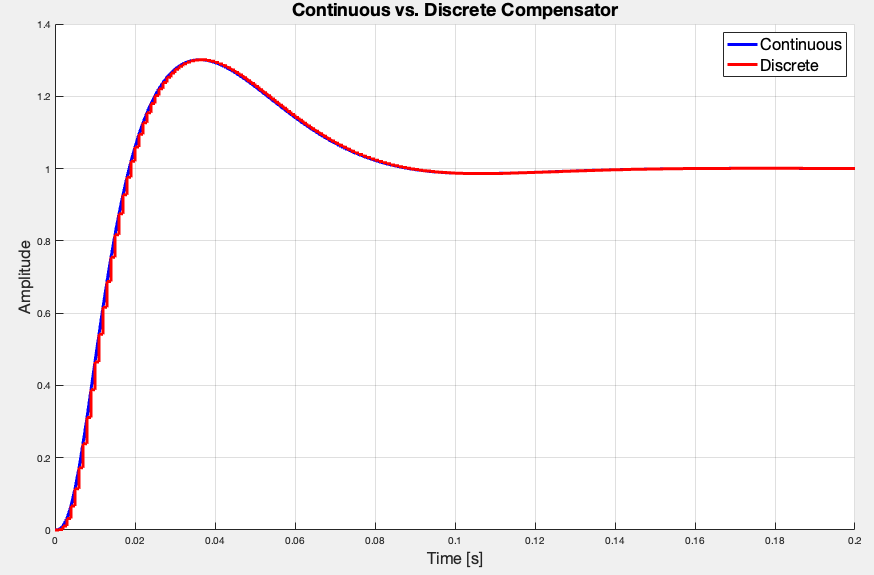
\includegraphics[width=0.75\textwidth]{p6.png}
    \caption{Equivalent Compensator Response.}
  \end{figure}

\end{enumerate}

\end{document}